\section{Integration Strategy}

This section describes the integration plan for the system to be developed. As stated in the previous section, each component must first undergo \textit{Unit Testing}.
The aim of this section is to verify the interactions between the modules of DREAM, it is also exploited the system's coexistence with others and tests the interface between modules, we firstly test components individually \textit{Unit Testing} and then combined to make a system \textit{System testing}.
Every time that it is needed to test a component which is used by other ones that have not been integrated yet, an artificial environment is necessary for each integration test; the environment consists of driver programs and test data.
It is also important to point out that in our system there are some external components, such as: \textbf{Database} and \textbf{ExternalAPIs}, and so they are directly exploited without having to implement them, however they're integrated as soon as possible in order to test whether their interfaces can communicated properly.
The following diagrams illustrate the integration process at the various levels of dependency.
(Note that it is not possible to apply a pure bottom-up approach due to the mutual dependency relationship between \textit{ExternalAPIs} and some high level components).
\begin{center}
    \begin{figure}[h!]
  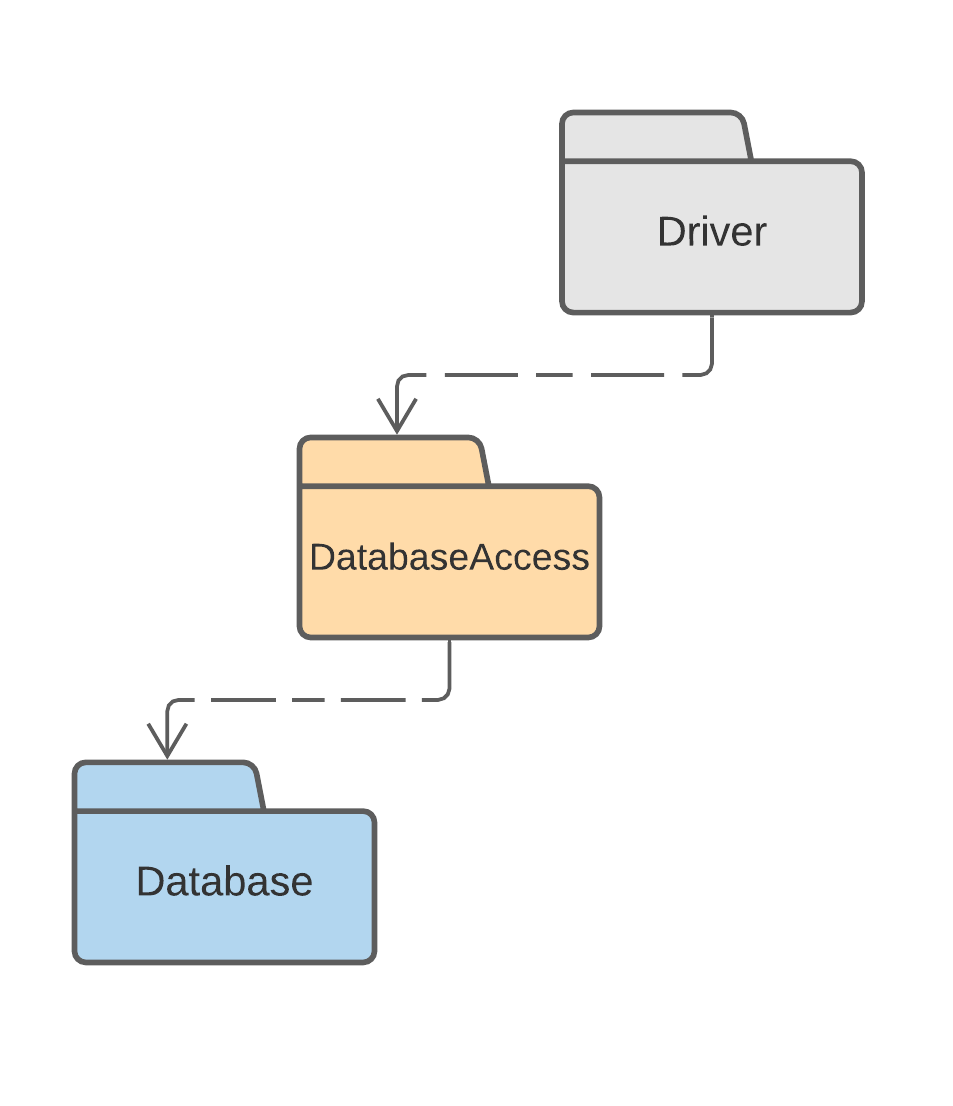
\includegraphics[width=\textwidth,height=\textheight,keepaspectratio]{./Images/IntegrationStrategy/IT1.png}
  \caption{integration of Database and DatabaseAccess components.}
\end{figure}
\end{center}


\begin{center}
    \begin{figure}[h!]
  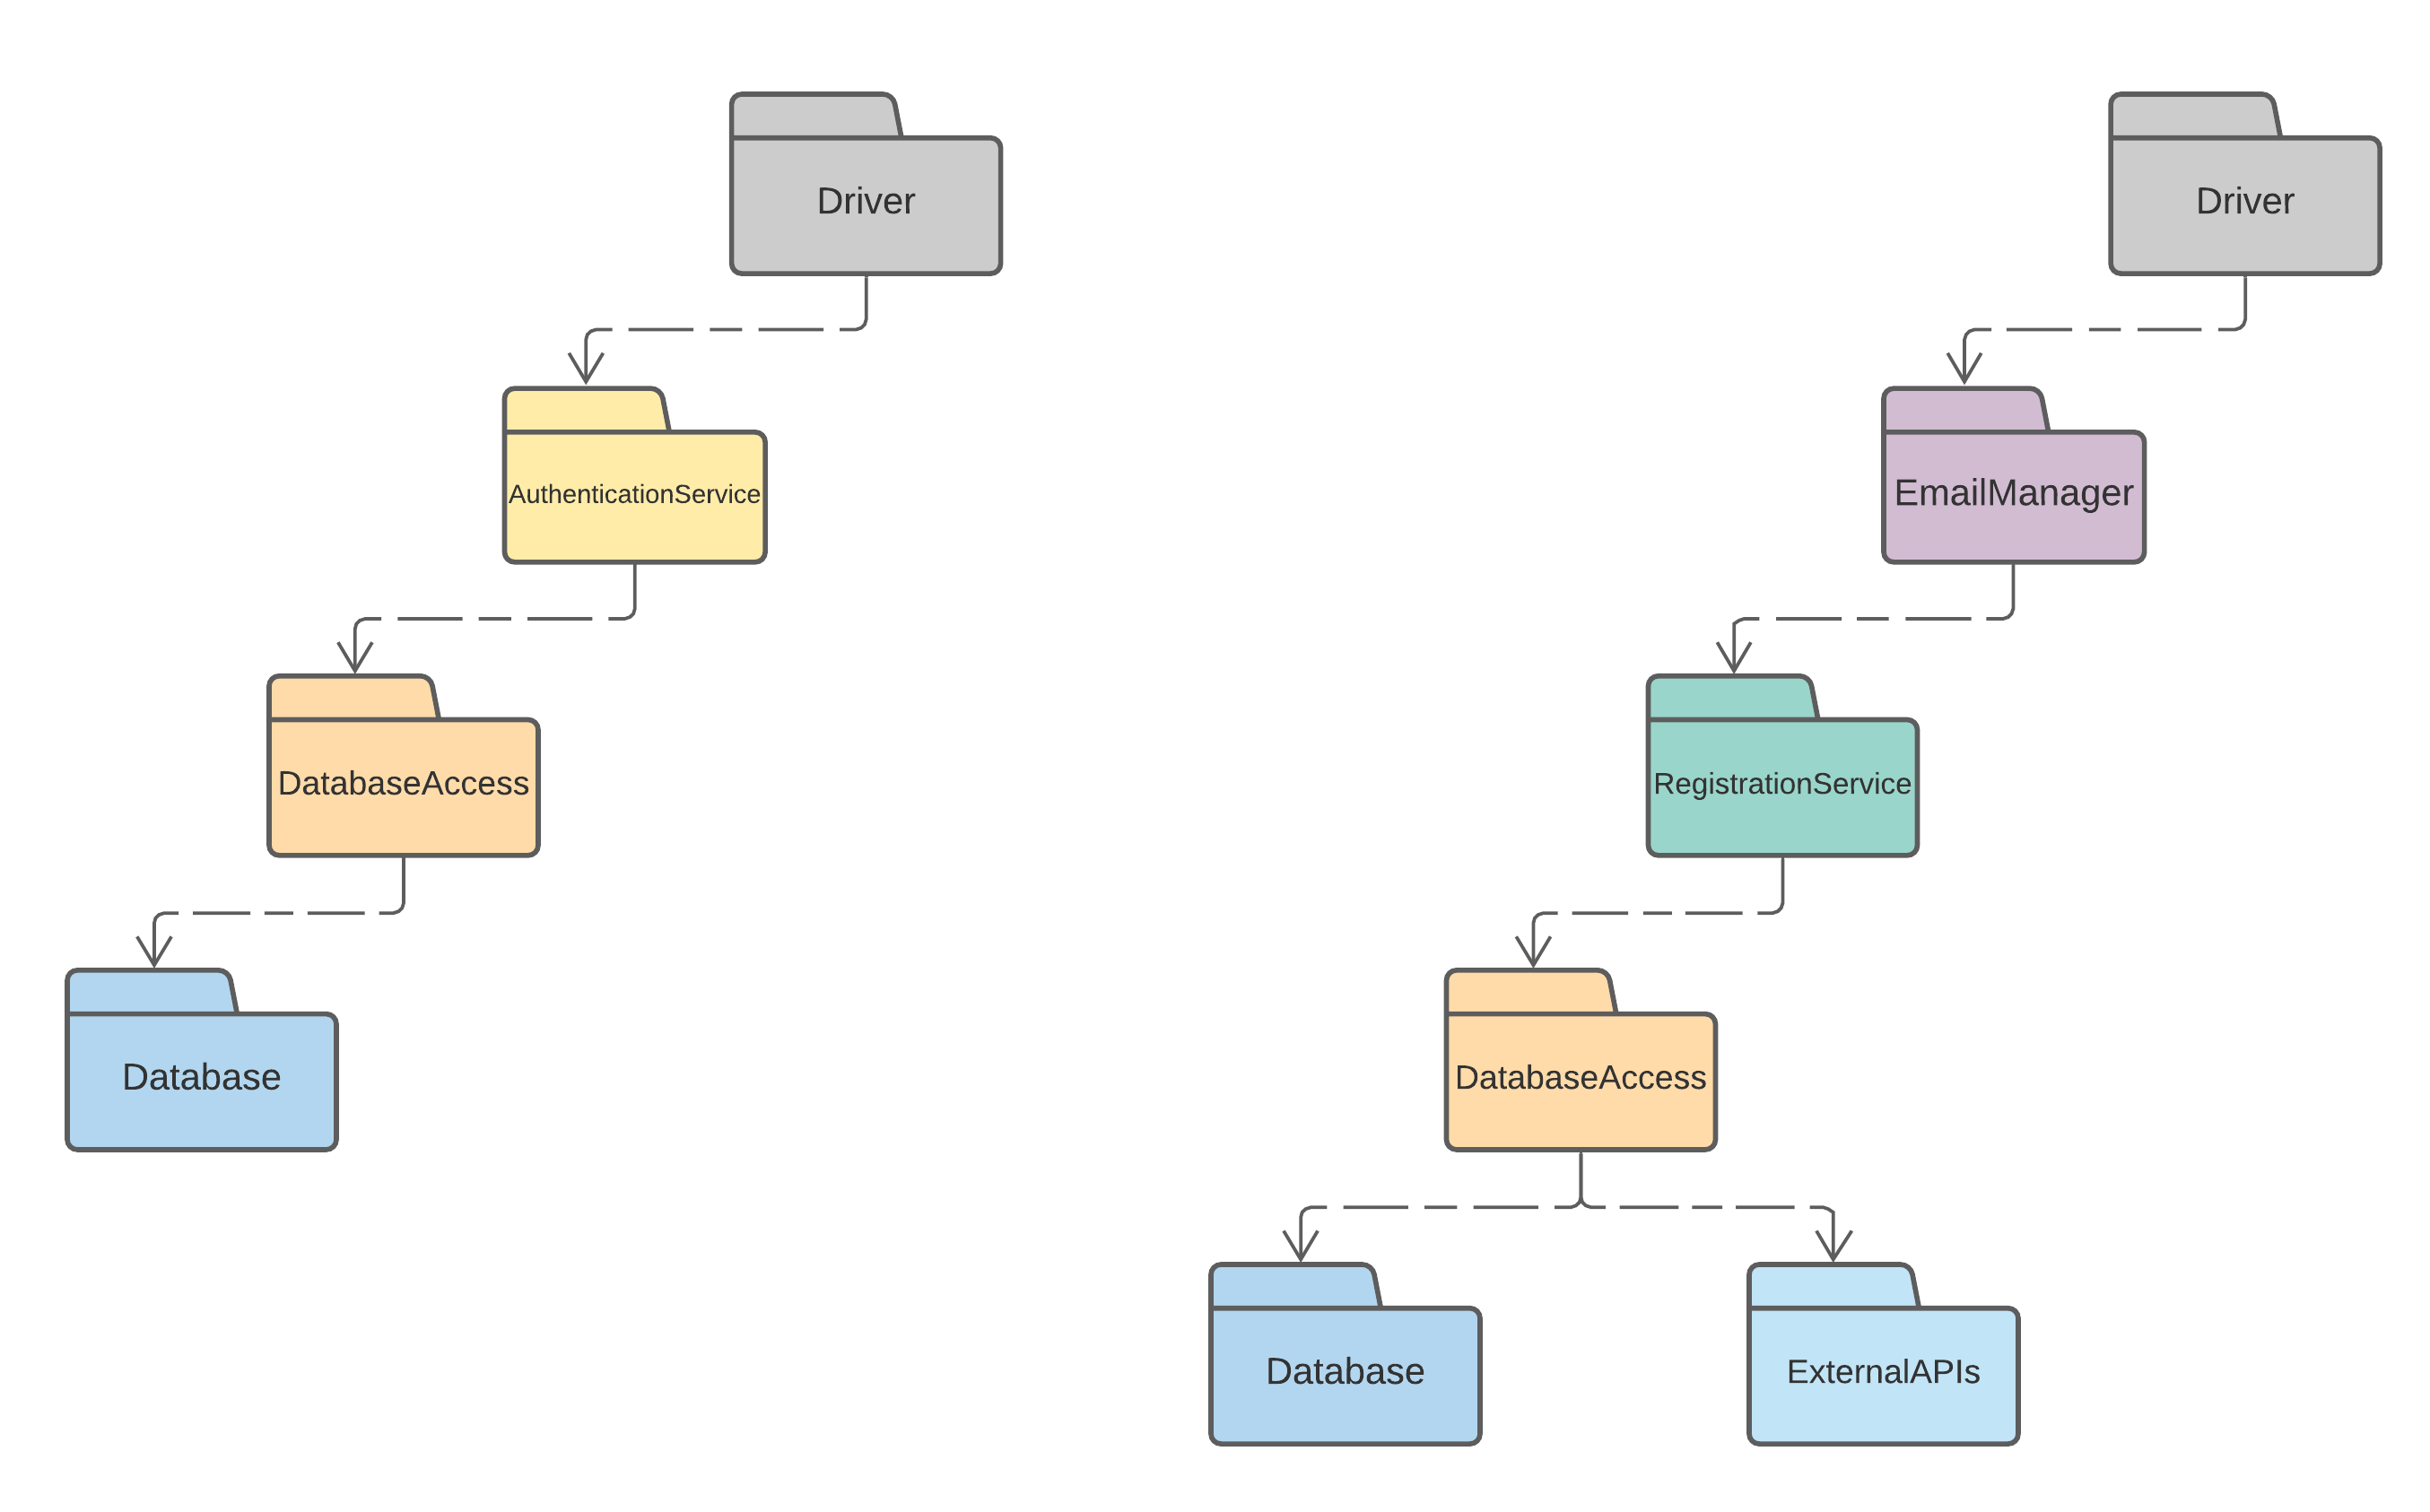
\includegraphics[width=\textwidth,height=\textheight,keepaspectratio]{./Images/IntegrationStrategy/IT2.png}
  \caption{Login and registration services integration.}
\end{figure}
\end{center}


\begin{center}
    \begin{figure}[h!]
  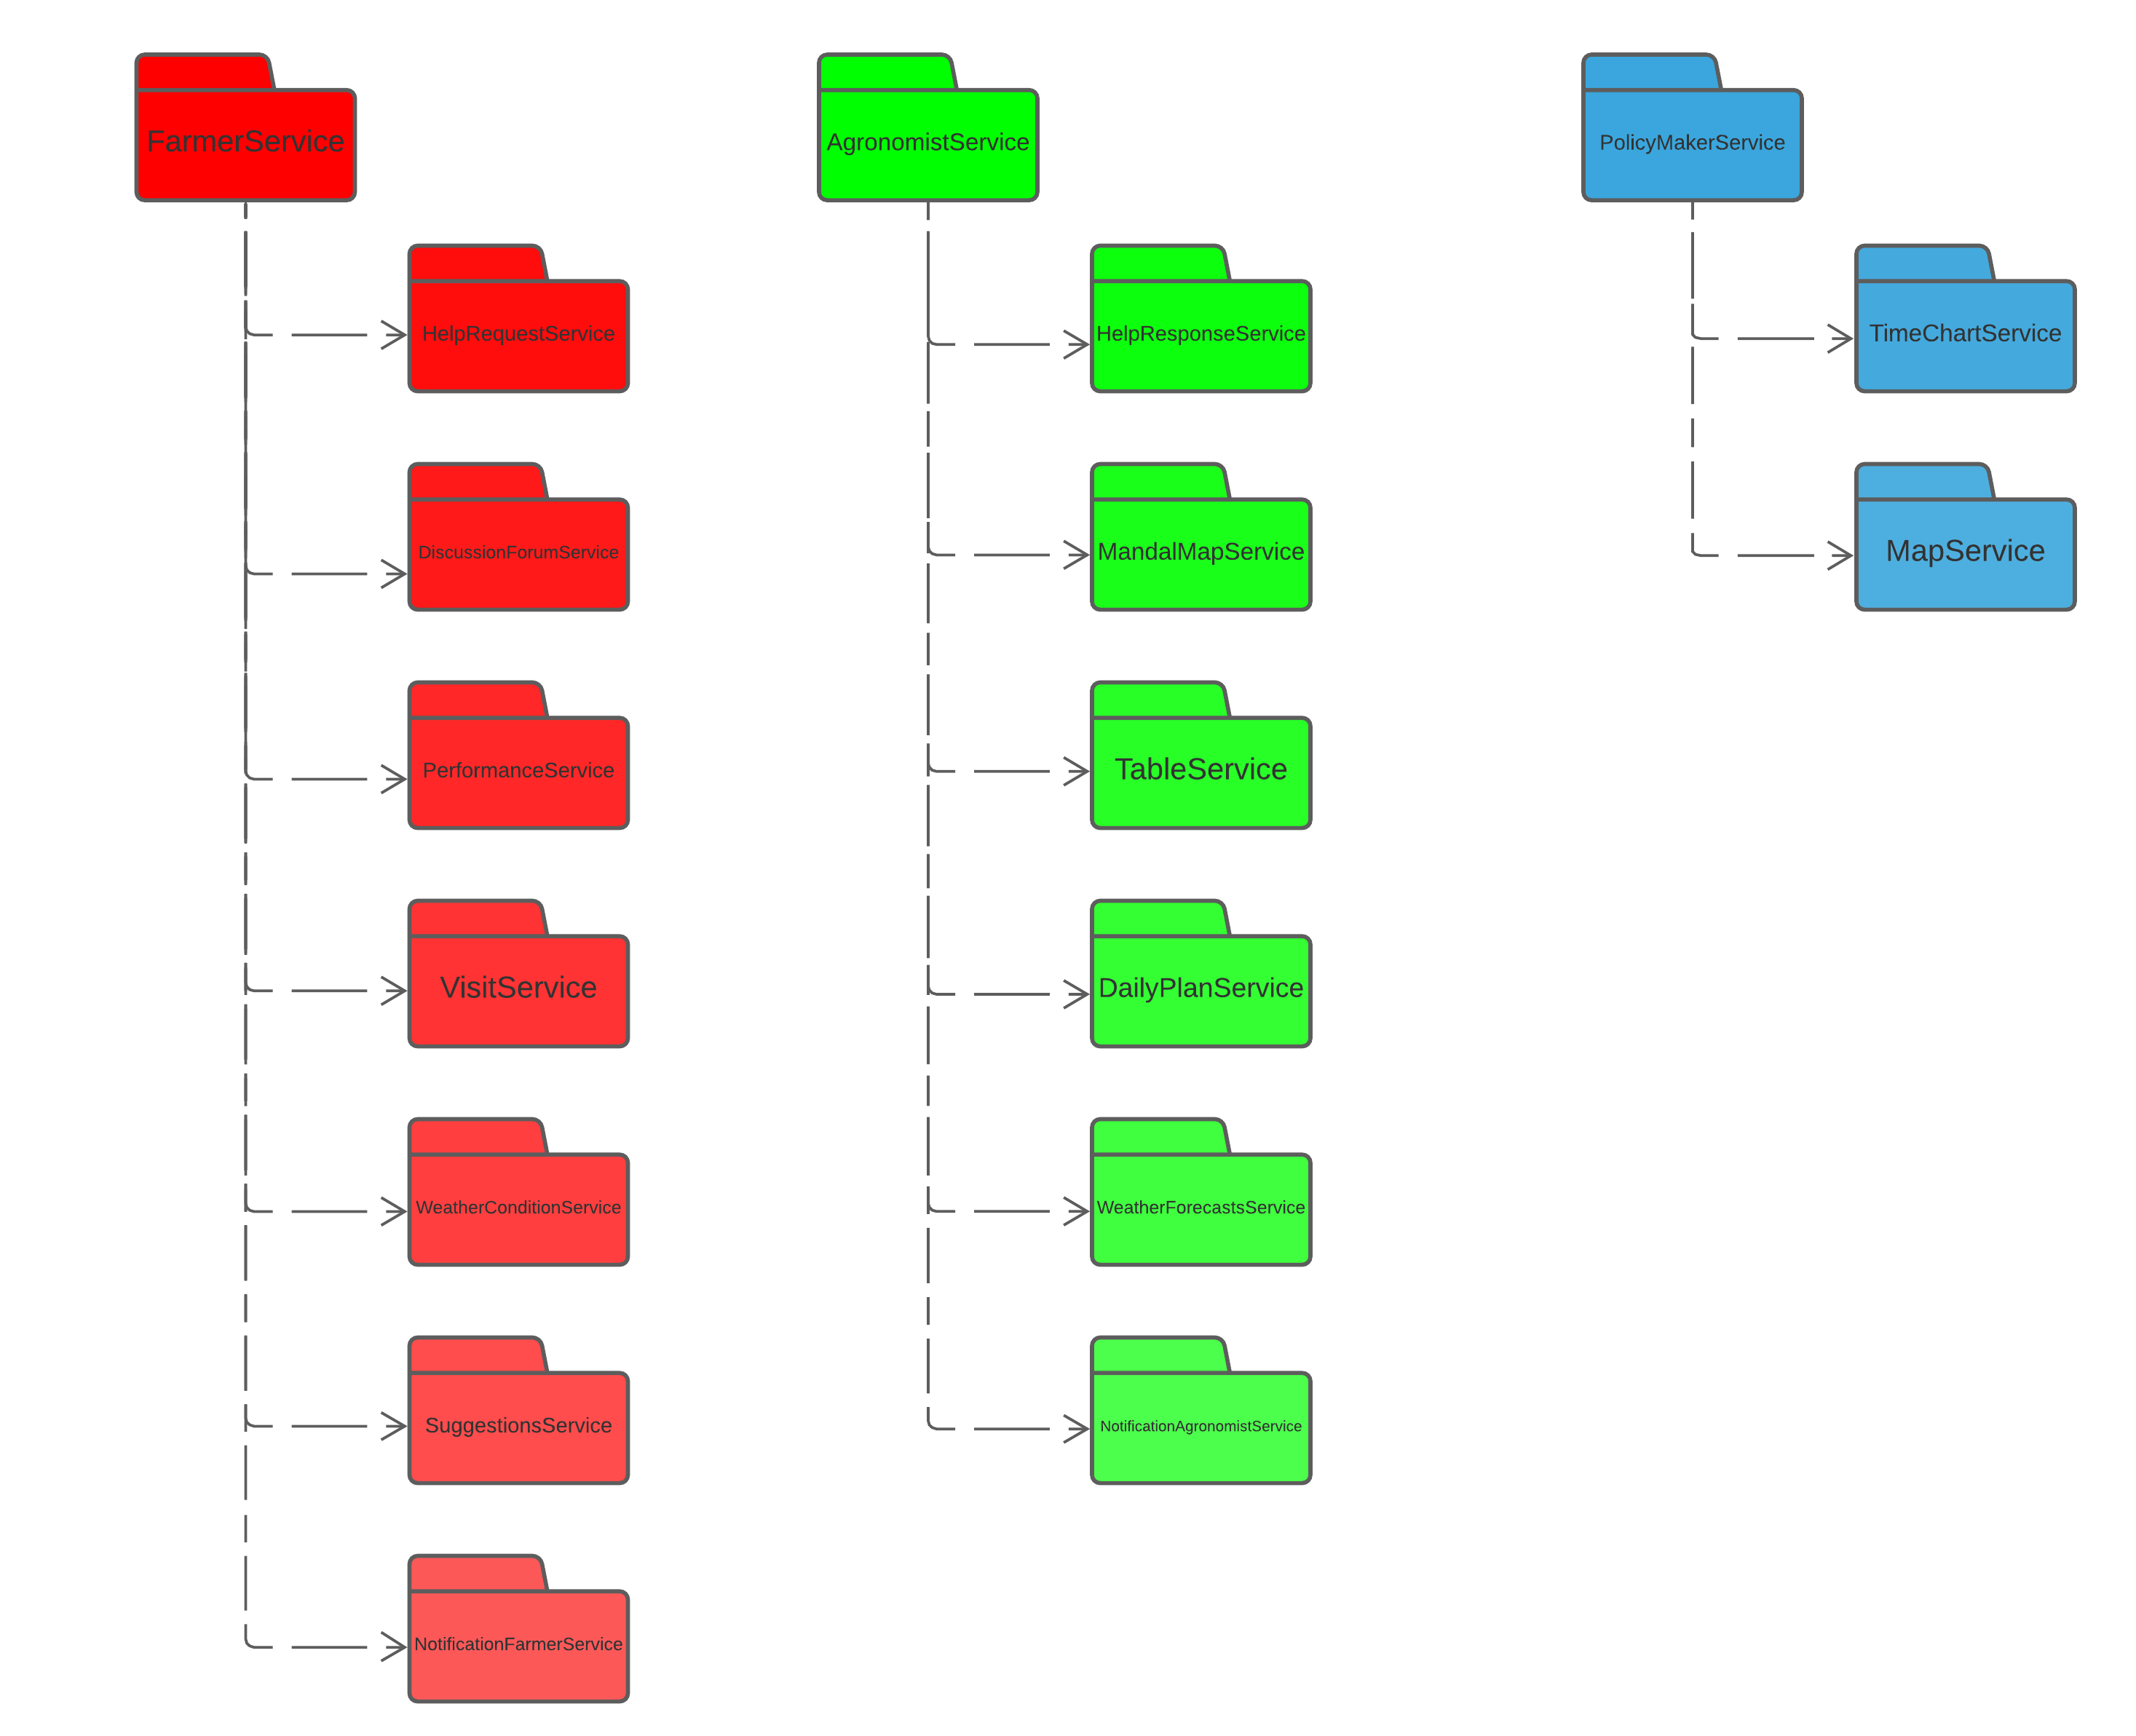
\includegraphics[width=\textwidth,height=\textheight,keepaspectratio]{./Images/IntegrationStrategy/IT3.png}
  \caption{Integration of components for the three actors}
\end{figure}
\end{center}



\begin{center}
    \begin{figure}[h!]
  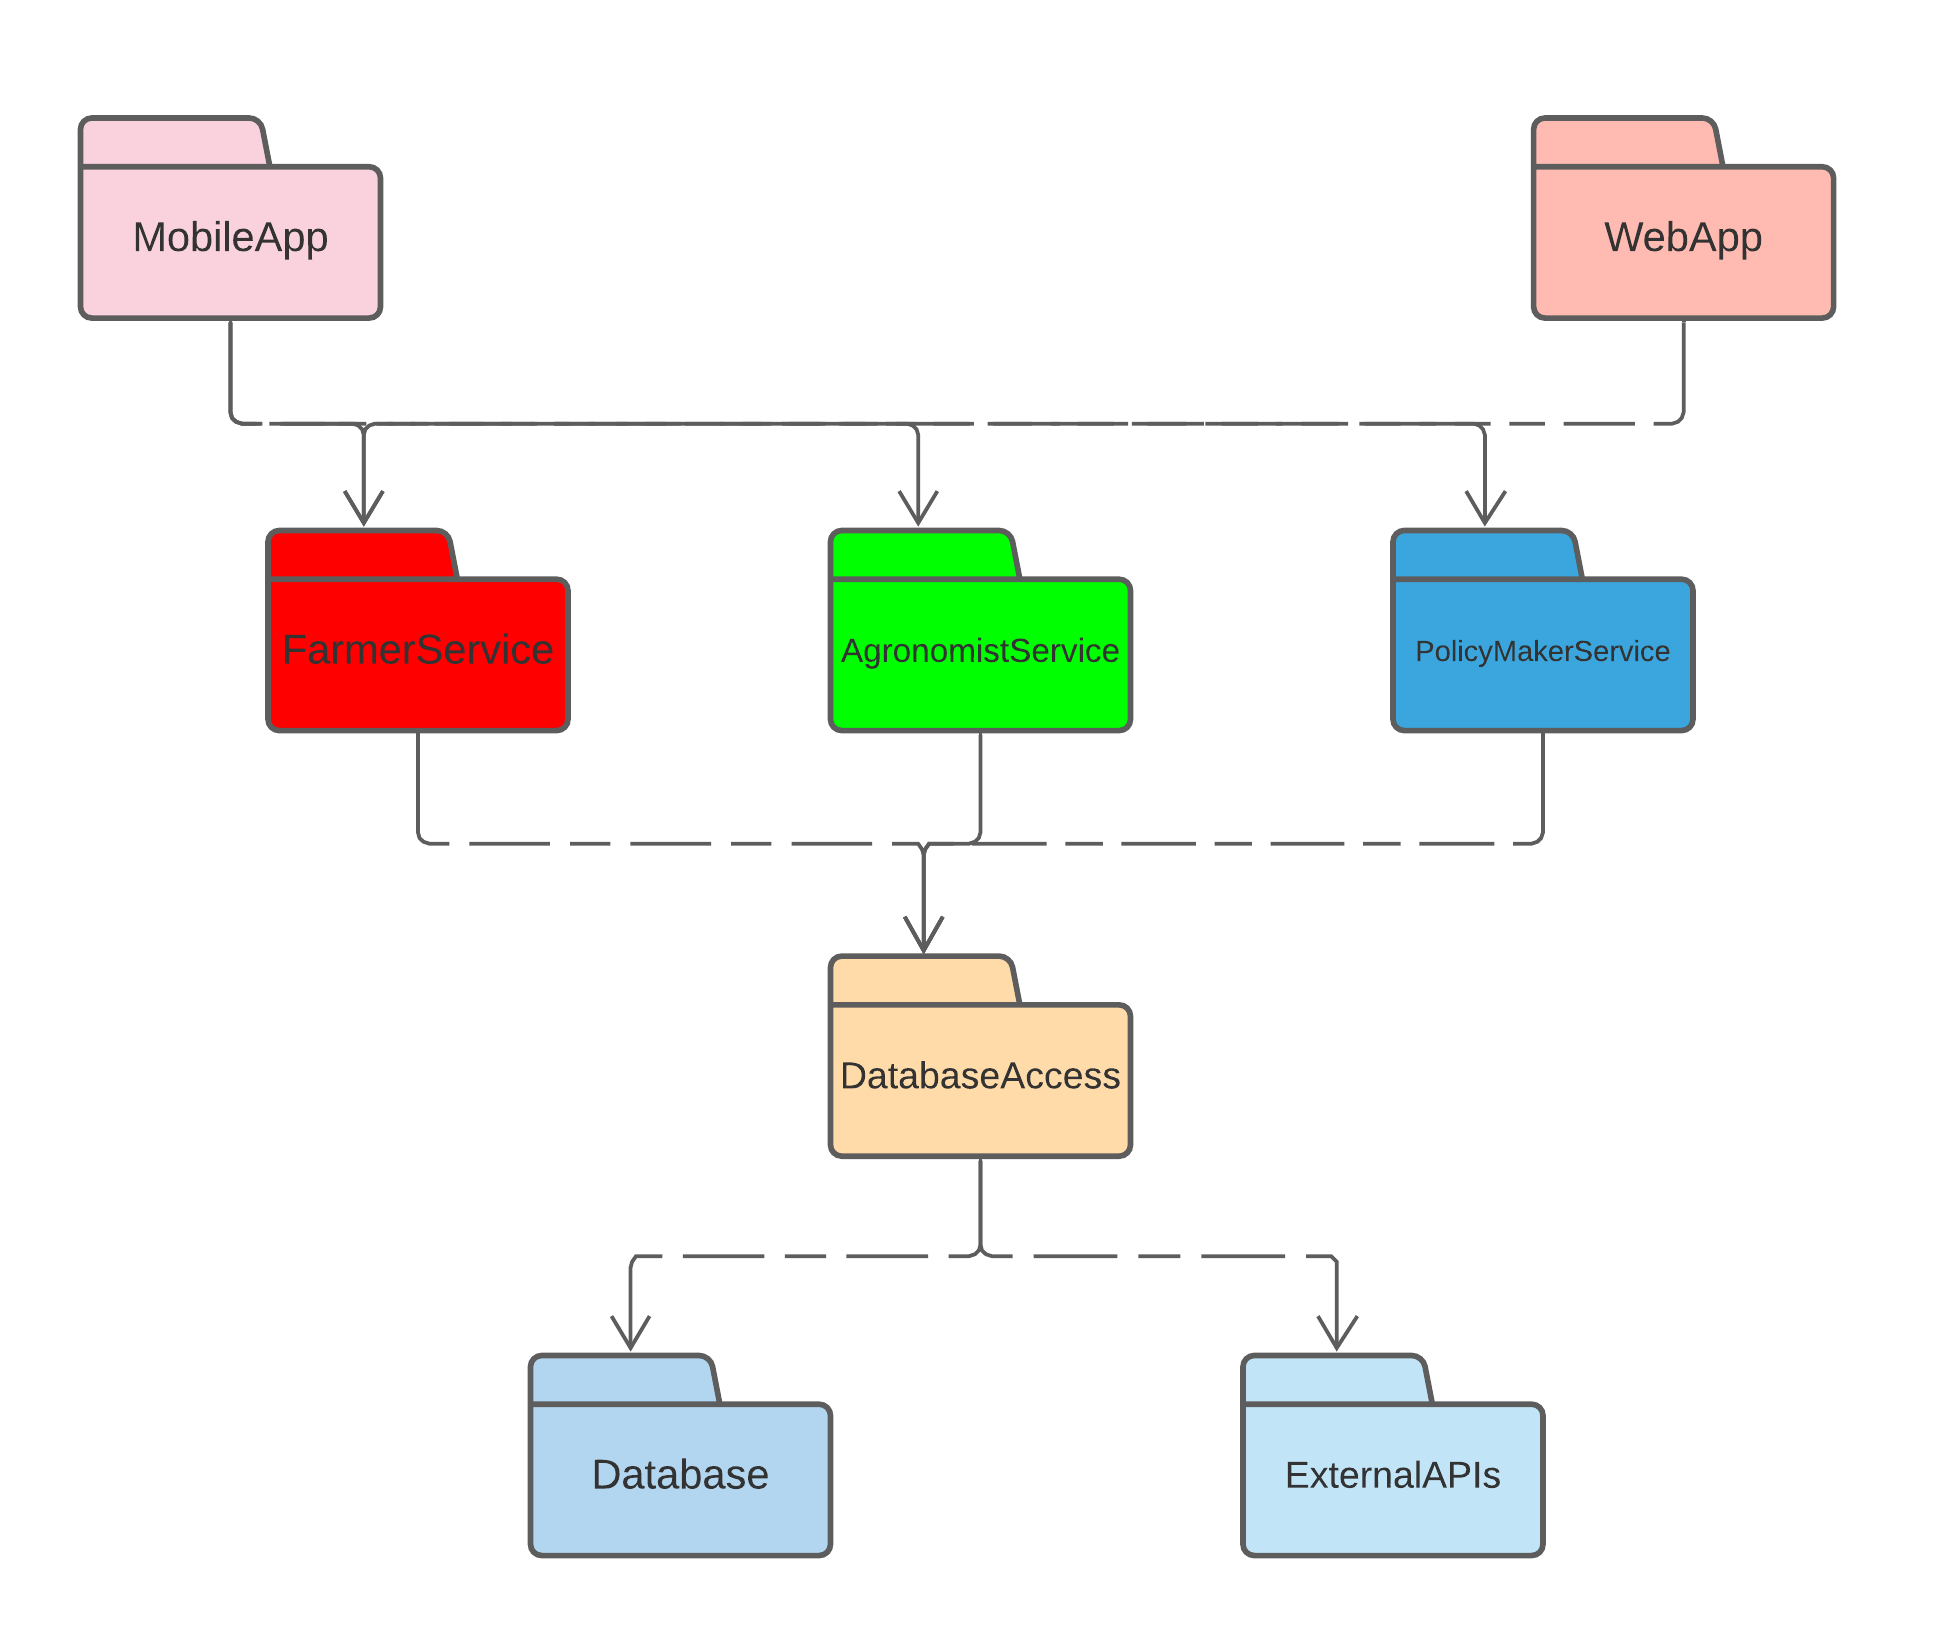
\includegraphics[width=\textwidth,height=\textheight,keepaspectratio]{./Images/IntegrationStrategy/IT4.png}
  \caption{Integration of all main components}
\end{figure}
\end{center}


\clearpage